\documentclass[14pt]{extarticle} 
\usepackage{amsmath,mathtools,amsfonts,amsthm,amssymb,hyperref}
\usepackage{wasysym,geometry,bussproofs,latexsym,parskip,bookmark}
\usepackage{mathtools,float}
\newtheorem{defn}{Definition}
\newtheorem{thm}{Theorem}
\newtheorem{claim}{Claim}
\newtheorem{lemma}{Lemma}
\hypersetup{colorlinks,allcolors=blue,linktoc=all}
\geometry{a4paper} 
\geometry{margin=0.5in}
\title{Math for CS 2015/2019 solutions to ``In-Class Problems Week 8, Fri. (Session 20)''}
\author{https://github.com/spamegg1}
\begin{document}
\maketitle
\tableofcontents

\section{Problem 1}
A portion of a computer program consists of a sequence of calculations where the results are stored in variables, like this:

\begin{center}
\begin{tabular}{rrcl}
& Inputs: & = & $a, b$ \\
Step 1.  & $c$ & = & $a+b$ \\
2. & $d$ & = & $a*c$\\
3. & $e$ & = & $c+3$\\
4. & $f$ & = & $c-e$\\
5. & $g$ & = & $a+f$\\
6. & $h$ & = & $f+1$\\
& Outputs: & & $d,g,h$
\end{tabular}
\end{center}

A computer can perform such calculations most quickly if the value of each variable is stored in a register, a chunk of very fast memory inside the microprocessor. Programming language compilers face the problem of assigning each variable in a program to a register. Computers usually have few registers, however, so they
must be used wisely and reused often. This is called the register allocation problem.

In the example above, variables $a$ and $b$ must be assigned different registers, because they hold distinct input values. Furthermore, $c$ and $d$ must be assigned different registers; if they used the same one, then the value of $c$ would be overwritten in the second step and we'd get the wrong answer in the third step. On the other hand, variables $b$ and $d$ may use the same register; after the first step, we no longer need $b$ and can overwrite the register that holds its value. Also, $f$ and $h$ may use the same register; once $f + 1$ is evaluated in the last step, the register holding the value of $f$ can be overwritten.

\subsection{(a)}
Recast the register allocation problem as a question about graph coloring. What do the vertices correspond to? Under what conditions should there be an edge between two vertices? Construct the graph
corresponding to the example above.
\begin{proof}
There is one vertex for each variable. An edge between two vertices indicates that the values of the variables must be stored in different registers.

We can classify each appearance of a variable in the program as either an assignment or a use. In particular, an appearance is an assignment if the variable is on the left side of an equation or on
the “Inputs” line. An appearance of a variable is a use if the variable is on the right side of an equation or on the “Outputs” line. The lifetime of a variable is the segment of code extending from the initial assignment of the variable until the last use (this definition is for the case that each variable is assigned at most once (see part (c))). There is an edge between two variables if their lifetimes overlap. This rule generates the following graph (next page):
\begin{figure}[ht!]
\centering
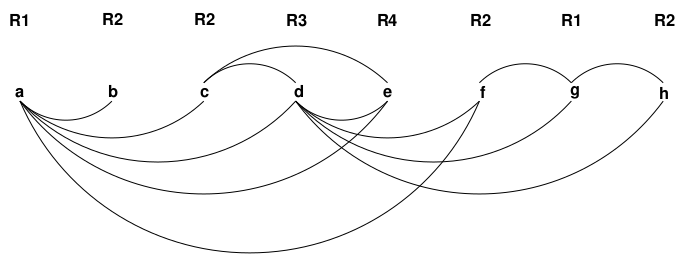
\includegraphics[scale=0.5]{register.png}
\end{figure}
\end{proof}
\subsection{(b)}
Color your graph using as few colors as you can. Call the computer's registers R1, R2, etc. Describe the assignment of variables to registers implied by your coloring. How many registers do you need?
\begin{proof}
Four registers (colors) are needed.

One possible assignment of variables to registers is indicated in the figure above. In general, coloring a graph using the minimum number of colors is quite difficult; no efficient procedure is
known. However, the register allocation problem always leads to an interval graph, and optimal colorings for interval graphs are always easy to find. This makes it easy for compilers to allocate
a minimum number of registers.
\end{proof}

\subsection{(c)}
Suppose that a variable is assigned a value more than once, as in the code snippet below:

\begin{center}
\begin{tabular}{ccc}
& $\ldots$ & \\
$t$ & = & $r+s$ \\
$u$ & = & $t*3$ \\
$t$ & = & $m-k$\\
$v$ & = & $t+u$\\
 & $\ldots$ &
\end{tabular}
\end{center}

How might you cope with this complication?

\begin{proof}
Each time a variable is reassigned, we could regard it as a completely new variable. Then we would regard the example as equivalent to the following:

\begin{center}
\begin{tabular}{ccc}
& $\ldots$ & \\
$t$ & = & $r+s$ \\
$u$ & = & $t*3$ \\
$t'$ & = & $m-k$\\
$v$ & = & $t'+u$\\
 & $\ldots$ &
\end{tabular}
\end{center}

We can now proceed with graph construction and coloring as before.
\end{proof}

\section{Problem 2}
{\bf False Claim.} {\it If every vertex in a graph has positive degree, then the graph is connected.}

\subsection{(a)}
Prove that this Claim is indeed false by providing a counterexample.
\begin{proof}
Consider $G = (V,E)$ where $V = \{a,b,c,d\}$ and $E = \{(a, b), (c, d)\}$. Every vertex has degree 1 but the graph is disconnected (it's split into two connected pieces $a-b$ and $c-d$).
\end{proof}

\subsection{(b)}
Since the Claim is false, there must be a logical mistake in the following bogus proof. Pinpoint the rst logical mistake (unjustified step) in the proof.

{\it Bogus proof.} We prove the Claim above by induction. Let $P(n)$ be the proposition that if every vertex in an $n$-vertex graph has positive degree, then the graph is connected.

{\bf Base cases:} $n \leq 2$. In a graph with 1 vertex, that vertex cannot have positive degree, so $P(1)$ holds vacuously.

$P(2)$ holds because there is only one graph with two vertices of positive degree, namely, the graph with an edge between the vertices, and this graph is connected.

{\bf Inductive step:} We must show that $P(n)$ implies $P(n + 1)$ for all $n \geq 2$. Consider an $n$-vertex graph in which every vertex has positive degree. By the assumption $P(n)$, this graph is connected; that is, there is a path between every pair of vertices. Now we add one more vertex $x$ to obtain an $n + 1$-vertex graph:

\begin{figure}[ht!]
\centering
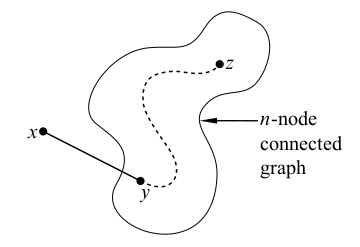
\includegraphics[scale=0.5]{n-node.png}
\end{figure}

All that remains is to check that there is a path from $x$ to every other vertex $z$. Since $x$ has positive degree, there is an edge from $x$ to some other vertex, $y$. Thus, we can obtain a path from $x$ to $z$ by going from $x$ to $y$ and then following the path from $y$ to $z$. This proves $P(n+1)$.

By the principle of induction, $P(n)$ is true for all $n \geq 0$, which proves the Claim.

\begin{proof}
This one is tricky: the proof is actually a good proof of something else. The first error in the proof is only in the final statement of the inductive step: “This proves $P (n + 1)$”.

The issue is that to prove $P (n + 1)$, every $(n + 1)$-vertex positive-degree graph must be shown to be connected. But the proof doesn’t show this. Instead, it shows that every $(n + 1)$-vertex positive-degree graph {\it that can be built up by adding a vertex of positive degree to an n-vertex connected graph}, is
connected.

The problem is that not every $(n + 1)$-vertex positive-degree graph can be built up in this way. The counterexample above illustrates this: there is no way to build that 4-vertex positive-degree graph from a 3-vertex positive-degree graph.

More generally, this is an example of “buildup error”. This error arises from a faulty assumption that every size $n + 1$ graph with some property can be “built up” in some particular way from a
size $n$ graph with the same property. (This assumption is correct for some properties, but incorrect for others, such as the one in the argument above.)

One way to avoid an accidental build-up error is to use a “shrink down, grow back” process in the inductive step: start with a size $n + 1$ graph, remove a vertex (or edge), apply the inductive
hypothesis $P (n)$ to the smaller graph, and then add back the vertex (or edge) and argue that $P (n + 1)$ holds. Let’s see what would have happened if we’d tried to prove the claim above by
this method:

{\bf Inductive step:} We must show that $P (n)$ implies $P (n + 1)$ for all $n \geq 1$. Consider an $(n + 1)$-vertex graph $G$ in which every vertex has degree at least 1. Remove an arbitrary vertex $v$, leaving an $n$-vertex graph $G'$ in which every vertex has degree... uh-oh! 

The reduced graph $G'$ might contain a vertex of degree 0, making the inductive hypothesis $P (n)$ inapplicable! We are stuck, and properly so, since the claim is false!
\end{proof}

\section{Problem 3}
In this problem, we examine an interesting connection between propositional logic and 3-colorings of certain
special graphs. Consider the graph in Figure 1. 

\begin{figure}[ht!]
\centering
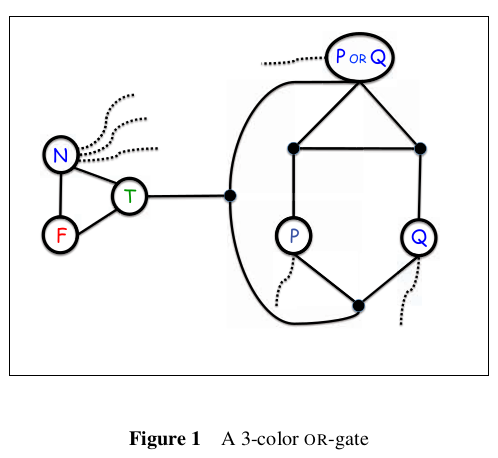
\includegraphics[scale=0.6]{3-color.png}
\end{figure}

We designate the vertices connected in the triangle on the left as {\it color-vertices}; since they form a triangle, they are forced to have different colors in any coloring of the graph. The colors assigned to the color-vertices will be called T, F and N. The dotted lines indicate edges between the color-vertex N, and the 3 other vertices $P$ OR $Q$, $P$, $Q$.

\subsection{(a)}
Prove that there exists a 3-coloring of the graph iff neither $P$ nor $Q$ are colored N.
\begin{proof}
1. Assume there exists a 3-coloring of the graph.

2. The color-vertex N is connected to the vertices $P$ and $Q$, therefore neither $P$ nor $Q$ is colored N.

3. Conversely, assume neither $P$ nor $Q$ is colored N. So there are 4 cases:

4. {\bf Case 1.} $P$ and $Q$ are both colored T.

Then we can color like this:

\begin{figure}[ht!]
\centering
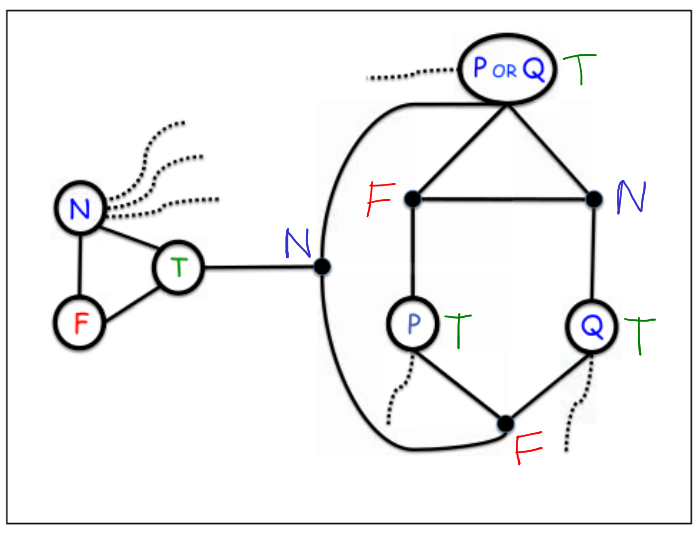
\includegraphics[scale=0.3]{3-color-1.png}
\end{figure}

5. {\bf Case 2.} $P$ and $Q$ are both colored F.

Then we can color like this:

\begin{figure}[ht!]
\centering
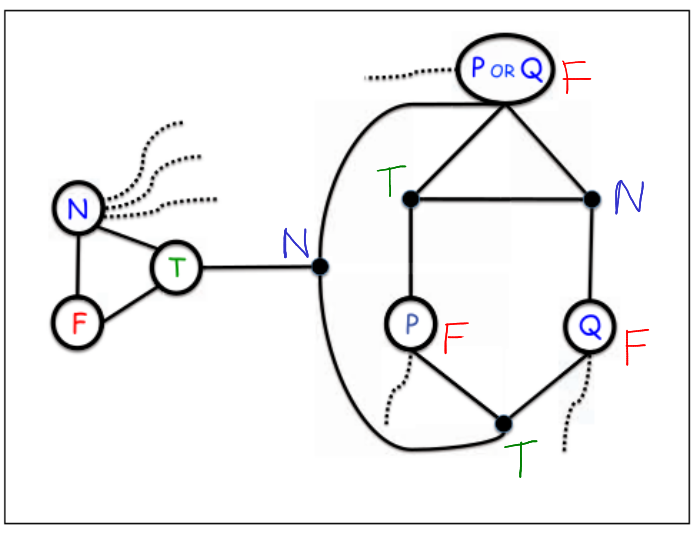
\includegraphics[scale=0.3]{3-color-2.png}
\end{figure}

6. {\bf Case 3.} $P$ is colored T, and $Q$ is colored F.

Then we can color like this:

\begin{figure}[ht!]
\centering
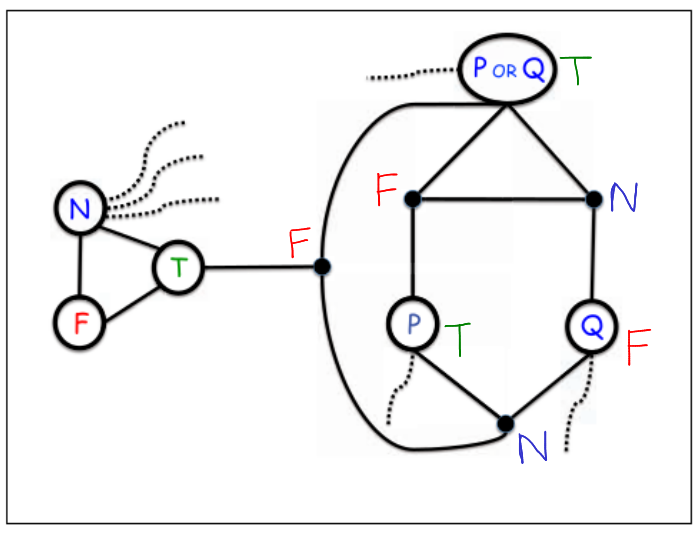
\includegraphics[scale=0.3]{3-color-3.png}
\end{figure}

7. {\bf Case 4.} $P$ is colored F, and $Q$ is colored T.

Then we can color like this:

\begin{figure}[ht!]
\centering
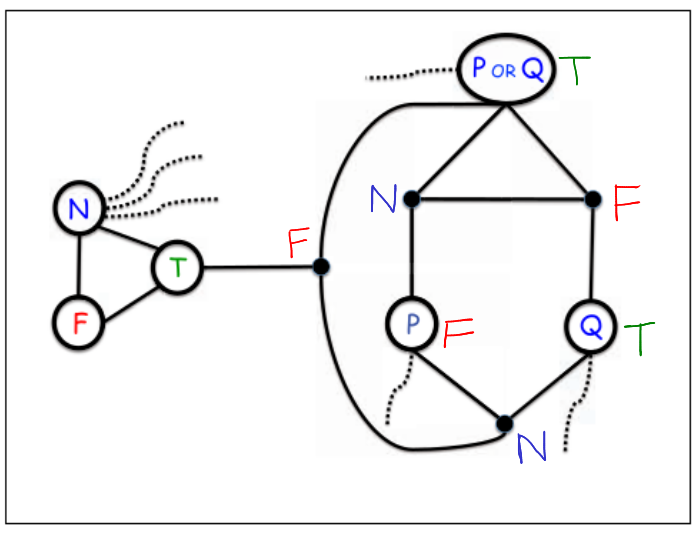
\includegraphics[scale=0.3]{3-color-4.png}
\end{figure}

\end{proof}

\subsection{(b)}
Argue that the graph in Figure 1 acts like a two-input OR-gate: a valid 3-coloring of the graph has the vertex labelled $P$ OR $Q$ colored T iff at least one of the vertices labelled $P$ and $Q$ are colored T.
\begin{proof}
1. Assume a valid 3-coloring of the graph has the vertex labelled $P$ OR $Q$ colored T.

2. Notice the vertex labelled $P$ OR $Q$ is on a triangle. So the other two vertices on the base of the triangle must be colored N and F. 

3. Notice the vertices labelled $P$ and $Q$ are connected to those two vertices of the triangle. 

4. Since those two vertices are labeled N and F by (2), we see that $P$ and $Q$ cannot be both colored F or both colored N, otherwise the 3-coloring would be invalid.

5. By part (a), neither $P$ nor $Q$ is colored N.

6. By (4) and (5) at least one of $P$ or $Q$ is colored T.

5. Conversely assume at least one of the vertices labelled $P$ and $Q$ are colored T (by some valid 3-coloring). 

Notice that since the vertex labelled $P$ OR $Q$ is connected to the color-vertex labeled N, it cannot be colored N. So $P$ OR $Q$ must be colored either T or F.

There are 3 cases:

6. {\bf Case 1.} Both $P$ and $Q$ are colored T.

Then the two vertices on the base of the top-right triangle must be colored F and N, which forces the vertex labelled $P$ OR $Q$ to be colored T.

7. {\bf Case 2.} $P$ is colored T, and $Q$ is colored F.

Then the vertex at the bottom right (connected to both $P$ and $Q$) must be colored N.

Then the vertex right in the center of the graph must be colored $F$.

The vertex labelled $P$ OR $Q$ is connected to that, so it must be labeled T.

8. {\bf Case 3.} $P$ is colored F, and $Q$ is colored T.

Same as in Case 2.
\end{proof}

\subsection{(c)}
Changing the endpoint of one edge in Figure 1 will turn it into a two-input AND simulator. Explain.
\begin{proof}
???
\end{proof}

\section{Problem 4}
The $n$-dimensional {\it hypercube}, $H_n$, is a graph whose vertices are the binary strings of length $n$. Two vertices are adjacent if and only if they differ in exactly 1 bit. For example, in $H_3$, vertices 111 and 011 are adjacent because they differ only in the first bit, while vertices 101 and 011 are not adjacent because they differ at both the first and second bits.

\subsection{(a)}
Verify that for any two vertices $x \neq y$ of $H_3$, there are 3 paths from $x$ to $y$ in $H_3$, such that, besides $x$ and $y$, no two of those paths have a vertex in common.
\begin{proof}
Define the distance between two binary strings of length n to be the number of positions at which they differ (this is known as the Hamming distance between the strings).

To show that there are 3 paths between any two distance 1 strings, we can, by symmetry, just consider paths between the vertices 000 and 001.

Paths from 000 to 001:

\begin{center}
\begin{tabular}{cccc}
& & 000 & 001 \\
000 & 010 & 011 & 001 \\
000 & 100 & 101 & 001 \\
\end{tabular}
\end{center}

Likewise for distance 2, it is enough to find paths between 000 and 011:

\begin{center}
\begin{tabular}{ccccc}
& & 000 & 010 & 011 \\
& & 000 & 001 & 011 \\
000 & 100 & 110 & 111 & 011 \\
\end{tabular}
\end{center}

Finally, for distance 3 from 000 to 111:

\begin{center}
\begin{tabular}{cccc}
000 & 001 & 011 & 111 \\
000 & 010 & 110 & 111 \\
000 & 100 & 101 & 111 \\
\end{tabular}
\end{center}

\end{proof}

\subsection{(b)}
Conclude that the connectivity of $H_3$ is 3.
\begin{proof}
Since there are three paths from $x$ to $y$ in $H_3$ that share no edges with one another, removing any two edges will leave one of these paths intact, so $x$ and $y$ remain connected. So removing two edges from $H_3$ does not disconnect it. On the other hand, removing all 3 edges incident to any vertex, disconnects that vertex. Thus the minimum number of edges necessary to disconnect $H_3$ is 3.
\end{proof}

\subsection{(c)}
Try extending your reasoning to $H_4$. (In fact, the connectivity of $H_n$ is $n$ for all $n \geq 1$. A proof appears in the problem solution.)

\begin{proof}
Two paths in a graph are said to cross when they have a vertex in common other than their endpoints. A set of paths in a graph don’t cross when no two paths in the set cross. A graph is $k$-routed if between every pair of distinct vertices in the graph there is a set of $k$ paths that don’t cross. We’ll show that

\begin{lemma}
$H_n$ is $n$-routed for all $n \geq 1$.
\end{lemma}

Since $H_n$ can be disconnected by deleting the $n$ edges incident to any vertex, this implies that $H_n$ has connectivity $n$.

The proof of the Lemma is by induction on $n$ with induction hypothesis:
$$
P(n) \Coloneqq H_n \text{ is $n$-routed}.
$$

{\bf Base case [$n = 1$]:} Since $H_1$ consists of two vertices connected by an edge, $P (1)$ is immediate.

{\bf Base case [$n = 2$]:} $H_2$ is a square. Vertices on opposite corners are obviously connected by two length 2 paths that don’t cross, and adjacent vertices are connected by a length 1 path and a length 3 path.

{\bf Inductive step:} We prove $P (n + 1)$ for $n \geq 2$ by letting $v$ and $w$ be two vertices of $H_{n+1}$ and describing $n + 1$ paths between them that don’t cross.

Let $R$ be any positive length path in $H_n$, say
$$
R = r0 , r1 , \ldots , rk
$$

For $b \in \{0, 1\}$ define the $H_{n+1}$ path
$$
bR \Coloneqq br_0 , br_1 , \ldots , br_k .
$$

{\bf Case 1:} The distance from $v$ to $w$ is $d \leq n$. In this case, the $(n + 1)$-bit strings $v$ and $w$ agree in one or more positions. By symmetry, we can assume without loss of generality that $v$ and $w$ both start with 0. That is $v = 0v'$ and $w = 0w'$ for some $n$-bit strings $v' , w'$. Now by induction, there are paths, $Q_i$ for $1\leq i \leq n$, that don’t cross going between $v'$ and $w'$ in $H_n$.

Define the first $n$ paths in $H_{n+1}$ between $v$ and $w$ to be
$$
\pi_i \Coloneqq 0Q_i
$$
for $1 \leq i \leq n$. These paths don’t cross since the $Q_i$’s don’t cross.

Then define the $n + 1$st path
$$
\pi_{n+1} \Coloneqq v, 1\pi_{v',w'}, w
$$

where $\pi_{v' ,w'}$ is any simple path from $v'$ to $w'$ in $H_n$ . Then $\pi_{n+1}$ obviously does not cross any of the other paths since $1\pi_{v',w'}$ is vertex disjoint from $0Q_i$ for $1 \leq i \leq n$.

This proves that $P (n + 1)$ hold in this case.

{\bf Case 2:} The distance from $v$ to $w$ is $n + 1$. By symmetry, we can assume without loss of generality that $v = 0^{n+1}$ and $w = 1^{n+1}$.

Now by induction, there are $n$ paths from $0^n$ to $1^n$ in $H_n$ that don’t cross in $H_n$. We can assume without loss of generality that each of these paths is simple.

Removing the shared first vertex, $0^n$, of these paths yields paths $R_1 , R_2 , \ldots , R_n$. Now the $R_i$’s are vertex disjoint except for their common endpoint, $1^n$. Let $s_i$ be the start vertex of the $R_i$ for $1 \leq i \leq n$.

We now define $n + 1$ paths in $H_{n+1}$ from $0^{n+1}$ to $1^{n+1}$ that don’t cross.

The first of these paths will be
$$
\pi_1 \Coloneqq 0^{n+1} , 10^n , 1R_1
$$

For $2 \leq i \leq n$, the $i$th of these paths will be
$$
\pi_i \Coloneqq 0^{n+1} , 0s_i , 1R_i 
$$

These paths don’t cross because:

the paths $1R_i$ for $1 \leq i \leq n$ are vertex disjoint except for their common endpoint, $1^{n+1}$ , because the $R_i$’s are vertex disjoint except for their common endpoint, $1^n$ ,

a vertex $0s_i$ does not appear on $\pi_j$ for any $j \neq i$ because the $s_i \neq s_j$ for $j \neq i$, and the other vertices on the $\pi_j$’s start with 1, 

the vertex $10^n$ appears only on $\pi_1$. This follows because if it appeared on $\pi_i$ for $i \neq 1$ it must appear on $1R_i$. That would imply that $0^n$ appears on $R_i$, contradicting the fact that the original path $0^n , R_i$ in $H_n$ is simple.

Finally, the $n + 1$st path will be
$$
\pi_{n+1} \Coloneqq 0^{n+1} , 0R_1 , 1^{n+1}
$$

Note that, since all but the final vertex on $\pi_{n+1}$ start with 0, the only vertices besides the endpoints that $\pi_{n+1}$ could share with another path would be $0s_i$ for $2 \leq i \leq n$. But none of these appear on $\pi_{n+1}$ because, except for their shared endpoint, $R_1$ is vertex disjoint from all the other $R_i$’s. 

This proves that $P (n + 1)$ holds in case 2, and therefore holds in all cases, which completes the proof by induction. 

Note that this proof implicitly defines a recursive procedure that, for any two vertices in $H_n$, finds between the two vertices $n$ simple paths of length at most $n + 1$ that don’t cross.
\end{proof}
\end{document}
